\section{Tatree\_\-base$<$ Sets\-Type $>$ Class Template Reference}
\label{class_tatree__base}\index{Tatree_base@{Tatree\_\-base}}
Template class representing a trie data structure.  


{\tt \#include $<$Tatree\_\-base.hxx$>$}

Inheritance diagram for Tatree\_\-base$<$ Sets\-Type $>$::\begin{figure}[H]
\begin{center}
\leavevmode
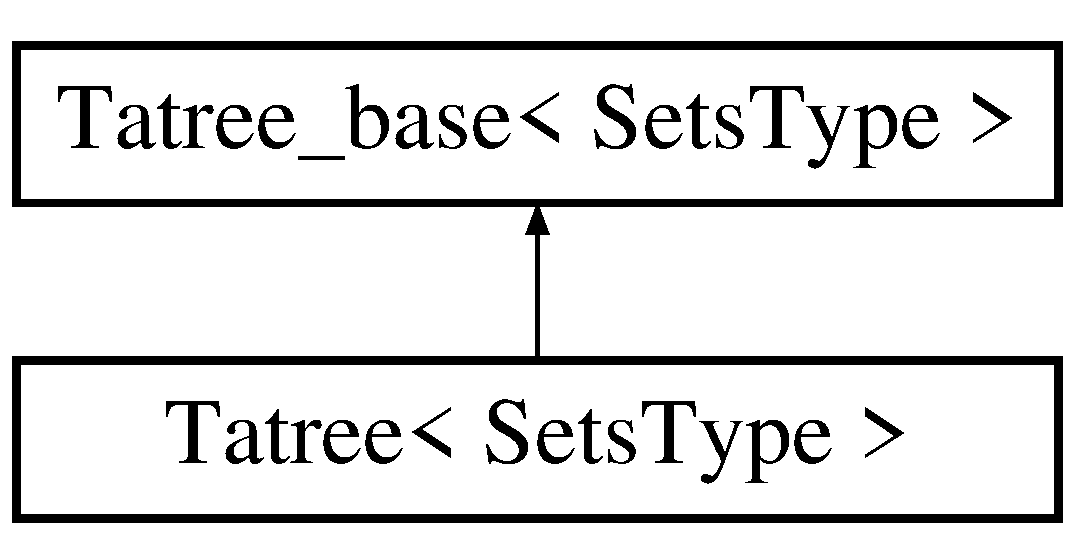
\includegraphics[height=2cm]{class_tatree__base}
\end{center}
\end{figure}
\subsection*{Public Types}
\begin{CompactItemize}
\item 
typedef {\bf It\-Tatree\_\-base}$<$ Sets\-Type $>$ {\bf iterator}\label{class_tatree__base_6f81c0610c9b60a3067eacc19fbe0190}

\begin{CompactList}\small\item\em Used to have the same syntax tha the STL. \item\end{CompactList}\end{CompactItemize}
\subsection*{Public Member Functions}
\begin{CompactItemize}
\item 
{\bf Tatree\_\-base} ()\label{class_tatree__base_c8206aefa793dc39fefa7d5112ac17a1}

\begin{CompactList}\small\item\em Constructor. \item\end{CompactList}\item 
{\bf $\sim$Tatree\_\-base} ()\label{class_tatree__base_0c831209dadbd62486cfcfc39864b5e7}

\begin{CompactList}\small\item\em Destructor. \item\end{CompactList}\item 
template$<$class Container$>$ void {\bf push\_\-back} (Container \&set\-Element, int nb=1)
\begin{CompactList}\small\item\em Push back a set of element in the trie. \item\end{CompactList}\item 
template$<$class Input\-Iterator$>$ void {\bf push\_\-back} (Input\-Iterator \&first, Input\-Iterator \&last, int nb=1)
\begin{CompactList}\small\item\em Push back a set of element in the trie. \item\end{CompactList}\item 
int {\bf size} ()\label{class_tatree__base_7b328d694667e2361991e7e39a911311}

\begin{CompactList}\small\item\em Function that returns the number of sets in the trie. \item\end{CompactList}\item 
{\bf It\-Tatree\_\-base}$<$ Sets\-Type $>$ {\bf begin} ()\label{class_tatree__base_5ac683d9ee2312f85017264dac63ff90}

\begin{CompactList}\small\item\em Return an iterator on the root node. \item\end{CompactList}\item 
{\bf It\-Tatree\_\-base}$<$ Sets\-Type $>$ {\bf begin\-Root} ()\label{class_tatree__base_b14eebc51ea7fc7afbfa3b1092cf093f}

\begin{CompactList}\small\item\em Return an iterator on the root node. \item\end{CompactList}\item 
{\bf It\-Tatree\_\-base}$<$ Sets\-Type $>$ {\bf end} ()\label{class_tatree__base_7021c1f8a67b2aea0d0f7675eb4a1167}

\begin{CompactList}\small\item\em Return an iterator on the element after the last element stored. \item\end{CompactList}\end{CompactItemize}
\subsection*{Protected Attributes}
\begin{CompactItemize}
\item 
{\bf Tatree\-Node}$<$ Sets\-Type $>$ $\ast$ {\bf root}\label{class_tatree__base_41ed3923edf2e25c6f9584a925e42291}

\begin{CompactList}\small\item\em Root node of the trie. \item\end{CompactList}\item 
{\bf Recode\-To\-Int}$<$ Sets\-Type $>$ $\ast$ {\bf recode}\label{class_tatree__base_4120099089ee2c29dd671e16aa7f5b3e}

\begin{CompactList}\small\item\em Functor used to recode and order elements. \item\end{CompactList}\item 
int {\bf nb\-Sets}\label{class_tatree__base_8a743634952a09c67867d0ed62c2b253}

\begin{CompactList}\small\item\em number of elements in the trie \item\end{CompactList}\end{CompactItemize}
\subsection*{Friends}
\begin{CompactItemize}
\item 
class {\bf It\-Tatree\_\-base$<$ Sets\-Type $>$}\label{class_tatree__base_1ce67181fc35f375e5115a7dfb1f0b3c}

\end{CompactItemize}


\subsection{Detailed Description}
\subsubsection*{template$<$class Sets\-Type$>$ class Tatree\_\-base$<$ Sets\-Type $>$}

Template class representing a trie data structure. 

The operations on a {\bf Tatree\_\-base}{\rm (p.\,\pageref{class_tatree__base})} are limited. For example, we cannot directly acces to the transactions by using ++ and $\ast$. The advantage of that type of structure is that it is lighter than one with more operations. Consequently code dedicated to such class will be more efficient.

The template parameter is the type of the element stored in the trie. 



\subsection{Member Function Documentation}
\index{Tatree_base@{Tatree\_\-base}!push_back@{push\_\-back}}
\index{push_back@{push\_\-back}!Tatree_base@{Tatree\_\-base}}
\subsubsection{\setlength{\rightskip}{0pt plus 5cm}template$<$class Sets\-Type$>$ template$<$class Input\-Iterator$>$ void {\bf Tatree\_\-base}$<$ Sets\-Type $>$::push\_\-back (Input\-Iterator \& {\em first}, Input\-Iterator \& {\em last}, int {\em nb} = {\tt 1})\hspace{0.3cm}{\tt  [inline]}}\label{class_tatree__base_6d855d39b3bdf83c4c759190d763e20a}


Push back a set of element in the trie. 

The template parameter represents the input iterators on the elements to insert in the trie. \begin{Desc}
\item[Parameters:]
\begin{description}
\item[{\em first}]iterator on the first element \item[{\em last}]iterator on the element after the last \item[{\em nb}]the number of times the set is inserted \end{description}
\end{Desc}
\index{Tatree_base@{Tatree\_\-base}!push_back@{push\_\-back}}
\index{push_back@{push\_\-back}!Tatree_base@{Tatree\_\-base}}
\subsubsection{\setlength{\rightskip}{0pt plus 5cm}template$<$class Sets\-Type$>$ template$<$class Container$>$ void {\bf Tatree\_\-base}$<$ Sets\-Type $>$::push\_\-back (Container \& {\em set\-Element}, int {\em nb} = {\tt 1})\hspace{0.3cm}{\tt  [inline]}}\label{class_tatree__base_66e0c0d2fa534d9cf53a9b5fe732eb79}


Push back a set of element in the trie. 

This function corresponds to the classic {\bf push\_\-back( )}{\rm (p.\,\pageref{class_tatree__base_66e0c0d2fa534d9cf53a9b5fe732eb79})} function od STL container. The template parameter represents a container of element of type Sets\-Type. \begin{Desc}
\item[Parameters:]
\begin{description}
\item[{\em set\-Element}]the set of element to insert in the trie \item[{\em nb}]the number of times the set is inserted \end{description}
\end{Desc}


The documentation for this class was generated from the following file:\begin{CompactItemize}
\item 
F:/i\-Zi/data\-Structures/trie/Tatree\_\-base.hxx\end{CompactItemize}
